\documentclass{standalone}

\usepackage[OT1]{fontenc}
\renewcommand*\familydefault{\sfdefault}
\usepackage{helvet,sfmath}
\usepackage{siunitx}

\usepackage{tikz}
\usetikzlibrary{arrows,calc,patterns}
% \usetikzlibrary{intersections, calc, arrows.meta}
\usepackage{tikz,tkz-euclide}

\begin{document}
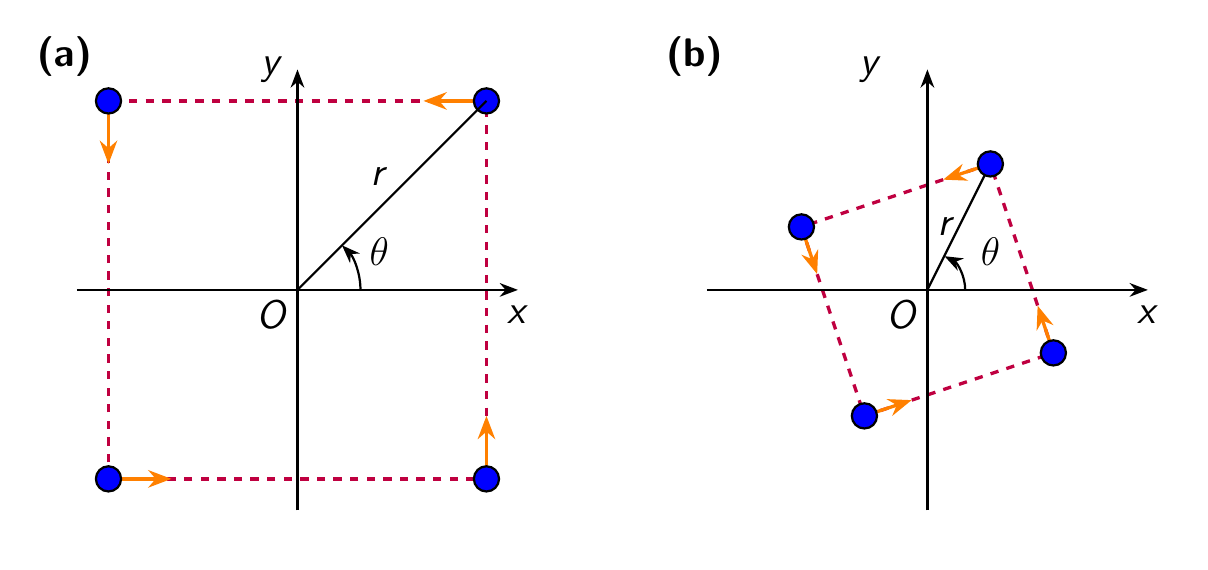
\begin{tikzpicture}[scale=0.8, >=Stealth]
    %% Background
    \draw[draw=none] (-9,-4) rectangle (9,4);

    %% Initial
    \draw[very thick, dashed, purple] (-8,-3) rectangle (-2,3);
    \draw[thick, ->] (-5,-3.5) to (-5,3.5);
    \draw[thick, ->] (-8.5,0) to (-1.5,0);

    \draw[very thick, orange,->] (-8,-3) to (-7,-3);
    \draw[very thick, orange,->] (-8,3) to (-8,2);
    \draw[very thick, orange,->] (-2,3) to (-3,3);
    \draw[very thick, orange,->] (-2,-3) to (-2,-2);
    
    \draw[thick, fill=blue]
    (-8,-3) circle (0.2)
    (-2,-3) circle (0.2)
    (-8,3) circle (0.2)
    (-2,3) circle (0.2)
    ;

    \draw[thick] (-5,0) to (-2,3);
    \draw[thick, ->] (-4,0) arc (0:45:1);
    
    \draw
    (-5.4,-0.4) node{\Large \(O\)}
    (-1.5,-0.4) node{\Large \(x\)}
    (-5.4,3.5) node{\Large \(y\)}
    (-3.7,1.8) node{\Large \(r\)}
    (-3.7,0.6) node{\Large \(\theta\)}
    ;

    %% At a random moment
    \draw[very thick, dashed, purple] (6,2) to (3,1) to (4,-2) to (7,-1) to (6,2);
    \draw[thick, ->] (5,-3.5) to (5,3.5);
    \draw[thick, ->] (1.5,0) to (8.5,0);
    \draw[thick] (5,0) to (6,2);
    \draw[thick, ->] (5.6,0) arc (0:63:0.6);

    \draw[very thick, orange,->] (6,2) to (5.25,1.75);
    \draw[very thick, orange,->] (3,1) to (3.25,0.25);
    \draw[very thick, orange,->] (4,-2) to (4.75,-1.75);
    \draw[very thick, orange,->] (7,-1) to (6.75,-0.25);

    \draw[thick, fill=blue]
    (6,2) circle (0.2)
    (3,1) circle (0.2)
    (4,-2) circle (0.2)
    (7,-1) circle (0.2)
    ;

    \draw
    (4.6,-0.4) node{\Large \(O\)}
    (8.5,-0.4) node{\Large \(x\)}
    (4.1,3.5) node{\Large \(y\)}
    (5.3,1) node{\Large \(r\)}
    (6,0.6) node{\Large \(\theta\)}
    ;

    \draw
    (-8.7,3.7) node{\Large \textbf{(a)}}
    (1.3,3.7) node{\Large \textbf{(b)}}
    ;
    
\end{tikzpicture}
\end{document}
